\thispagestyle{empty}

\hfill

\vfill

\noindent
This document was typeset using \LaTeX~and the typographical look-and-feel \texttt{classicthesis} developed by Andr\'e Miede.
 
The style was inspired by Robert Bringhurst's seminal book on typography ``\emph{The Elements of Typographic Style}''.\\

\noindent
Cover design by Paul Verspaget, Verspaget \& Bruinink\\

\noindent
Printed by Eindhoven University Press\\

\begin{wrapfigure}{l}{2.2cm} % "placement and width parameter for the width of the image space.
\centering
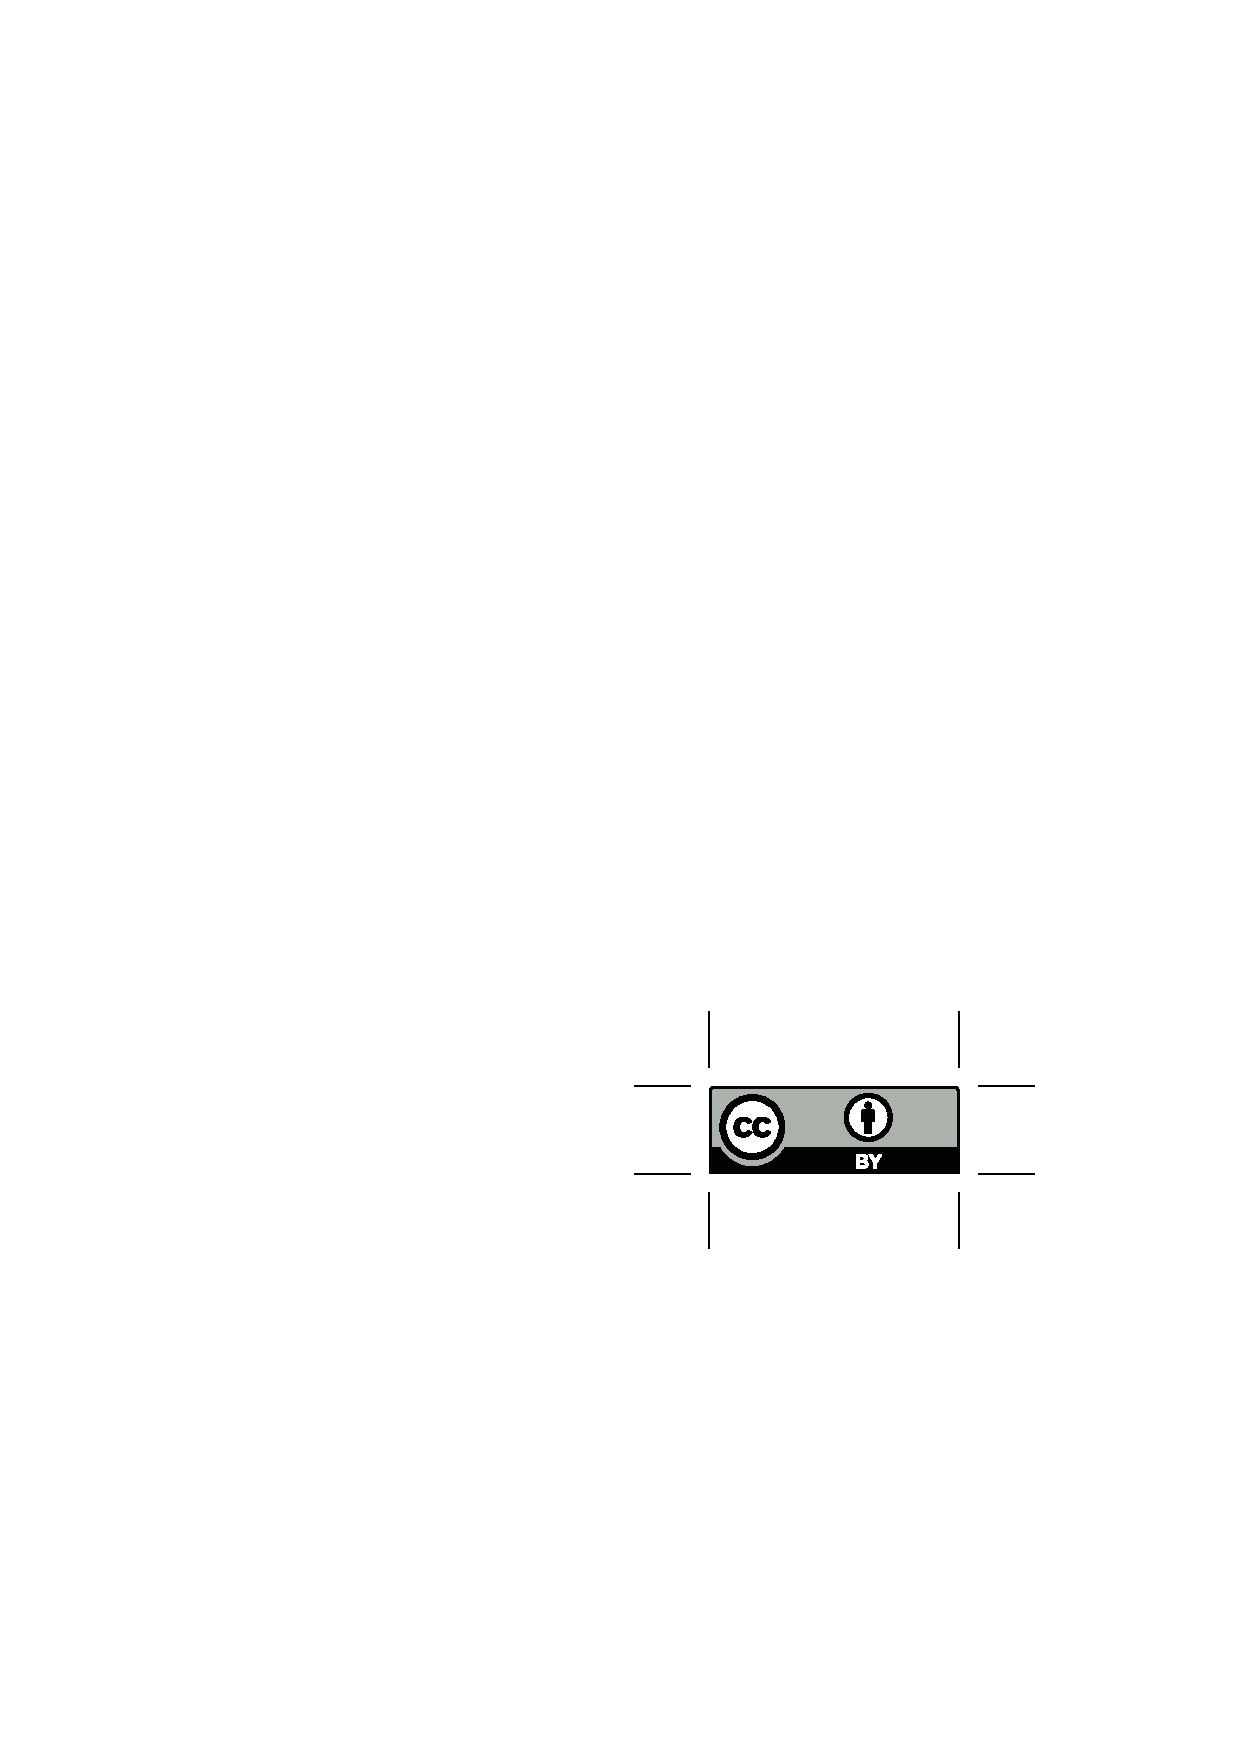
\includegraphics[width=2cm]{by}
\end{wrapfigure}

\noindent
``iPhone'', ``Alarm Clock'', ``Computer'' and ``Wireless'' symbols by The Noun Project, from The Noun Project collection.\\
``A graphic language for touch'', Timo Arnall.\\

\begin{wrapfigure}{l}{2.2cm} 
\centering

\includegraphics[width=2cm]{cc-zero}
\end{wrapfigure}

\noindent
``Desk Lamp'' symbol by Edward Boatman, ``Radio'' symbol by National Park Service, ``User'' symbol by Denis Chenu, ``Music'' symbol by Ryan Oksenhorn, from The Noun Project collection.\\


\noindent\myName: \textit{\myTitle,} \mySubtitle, %\myDegree, 
\textcopyright\ \myTime\\

\noindent
A catalogue record is available from the Eindhoven University of Technology Library.\\
ISBN: \\

\noindent
Proefontwerp Technische Universiteit Eindhoven\\
Trefw.: Ontologies, Semantic Web, Software Architecture, Interaction Design


%\bigskip
%
%\noindent\spacedlowsmallcaps{Supervisors}: \\
%\myProf \\
%\myOtherProf \\ 
%\mySupervisor
%
%\medskip
%
%\noindent\spacedlowsmallcaps{Location}: \\
%\myLocation
%
%\medskip
%
%\noindent\spacedlowsmallcaps{Time Frame}: \\
%\myTime
